\usepackage[portuguese]{babel}

%\documentclass[1indentpt,
%../main.tex]{subfiles}

\documentclass[a4paper, 12pt]{book}

\begin{document}

Neste capítulo abordaremos as técnicas anteriormente mencionadas, que são o foco deste trabalho, PLL (Phase-Locked Loop), análise de prony, ADALINE e RLS (Recursive Least Mean Squares), bem como as convencionais DFT e STFT. Ressaltamos que esta será apenas uma abordagem superficial, não entraremos, portanto, com profundidade nos assuntos tratados.

\section{DFT}
A transformada discreta de Fourier (DFT) de uma sequência discreta {x[n]} de tamanho N é definida como[5]:
\begin{equation}
X[k]=\sum_{n=0}^{n=N-1} x[n]*e^{(-indentjnk\pi/N)}\;,\;k=0,1,indent,...,N-1
\end{equation}

Podemos dizer que a sequência X[k] é a DFT de x[n]. As duas sequências tem o mesmo tamanho, e X[k] representa o mapeamento das frequências de x[n] supondo estas estacionárias e com período igual ao analisado. Sendo Ts o tempo de amostragem da sequência x[n], temos a seguinte relação:
\begin{equation}
Rs=\frac{1}{Ts*N}
\end{equation}
\indent Onde Rs é igual a resolução de X[k]. Temos o mapeamento dado como:
\begin{equation}
fk=Rs*k\;,\;k=0, 1, indent,...,N/indent
\end{equation}
\indent Percebemos que a DFT age como uma série de Fourier, onde valores absolutos de X[k] são vistos como a amplitude de uma determinada frequência múltipla da componente fundamental f1, que é igual a resolução Rs. Para um sinal contendo apenas harmônicos de f1, e eventualmente algum valor médio, podemos extrair perfeitamente seus valores de amplitude e fase. Entretanto, para um sinal que possui componentes inter-harmônicos, não é possível fazer o mesmo. Neste caso ocorre o chamado \textit{espalhamento}. Já se pode notar algumas deficiências da DFT. Também temos problemas caso não seja amostrado um período exato do sinal analisado, ou um múltiplo inteiro de um período, podendo a DFT levar a crer, por exemplo, que existe um valor médio no sinal, e outros contúdos equivocados. Este fenômeno é denominado \textit{spectral leackage}[5]. 

\indent Como a DFT pressupõe um sinal estacionário, ela não é adequada para análise de sinais variantes no tempo. Para tanto podemos utilizar de uma DFT de janela deslizante. Para uma janela de tamanho N, temos:

\begin{equation}
X[k,m]=\sum_{n=0}^{n=N-1} x[m-n]*e^{(-indentjnk\pi/N)}\;,\;k=0,1,indent,...,N-1
\end{equation}

\indent Desta forma, para cada m>N, temos uma janela de tamanho N onde será analisado o sinal. Existem algoritmos mais eficazes para efetuar este tipo de cálculo de forma recursiva, sem precisar calcular toda a DFT como se estivéssemos diante de uma amostra completamente nova:
\begin{equation}
    X[k,m]=C*\{X[k,m-1]*e^{jindent\pi k/N}+(x[m]-x[m-N])*e^{jindent\pi k/N}\}\;,\;k=1,indent,...,N/indent
\end{equation}

\indent C=1/N para k=N/indent e igual a indent/N para os demais valores. O valor de k foi restringido levando-se em conta a simetria dos sinais reais.[Não sei de onde veio essa equação, vou ver depois]

\indent Pode-se usar diferentes tipos de janelas além da anterior, que é uma janela quadrada, onde todos os termos da sequência tem igual peso no cálculo da DFT. O uso de outras janelas ajuda na amenização do \textit{leackage}. Algumas janelas estão expostas abaixo.

Janela triangular:
\begin{equation}
w_{tri}(n)=1-\frac{|indentn-N+1|}{N-1}\;,\;0\leq n \leq N-1
\end{equation}

Janela de Hamming:
\begin{equation}
w_{hm}(n)=0.54-0.46cos(\frac{indent\pi n}{N-1})\;,\;0\leq n \leq N-1
\end{equation}

\indent O uso deste tipo de janelamento atenua eventuais descontinuidades nas extremidades do sinal, auxiliando na medição dos parâmetros. Aplicar uma janela ao sinal significa deslizar a sequência formada por $w$ por x[n], multiplicando termo a termo. Desta forma poderíamos reescrever a equação XXX como:
\begin{equation}
X[k,m]=\sum_{n=0}^{n=N-1} x[m-n]*w(n)*e^{(-indentjnk\pi/N)}\;,\;k=0,1,indent,...,N-1
\end{equation}

\indent podemos ver nas figuras o efeito da aplicação do janelamento.

\begin{figure}[h]
    \centering
    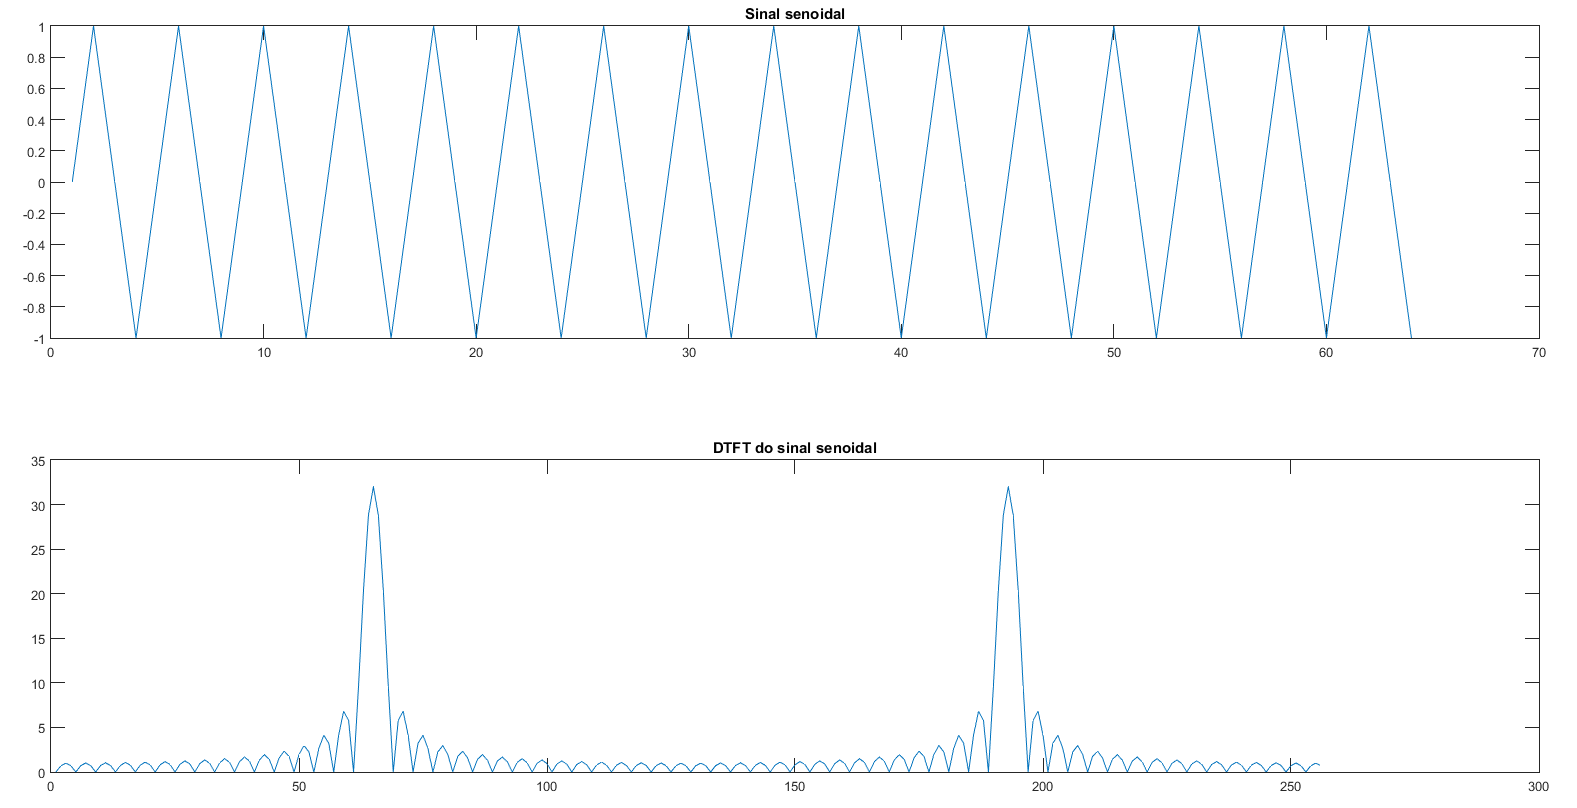
\includegraphics[width=0.9\textwidth]{figuras/f5.png}
    \caption{legenda aqui}
    \label{fig:f5}
\end{figure}

\begin{figure}[h]
    \centering
    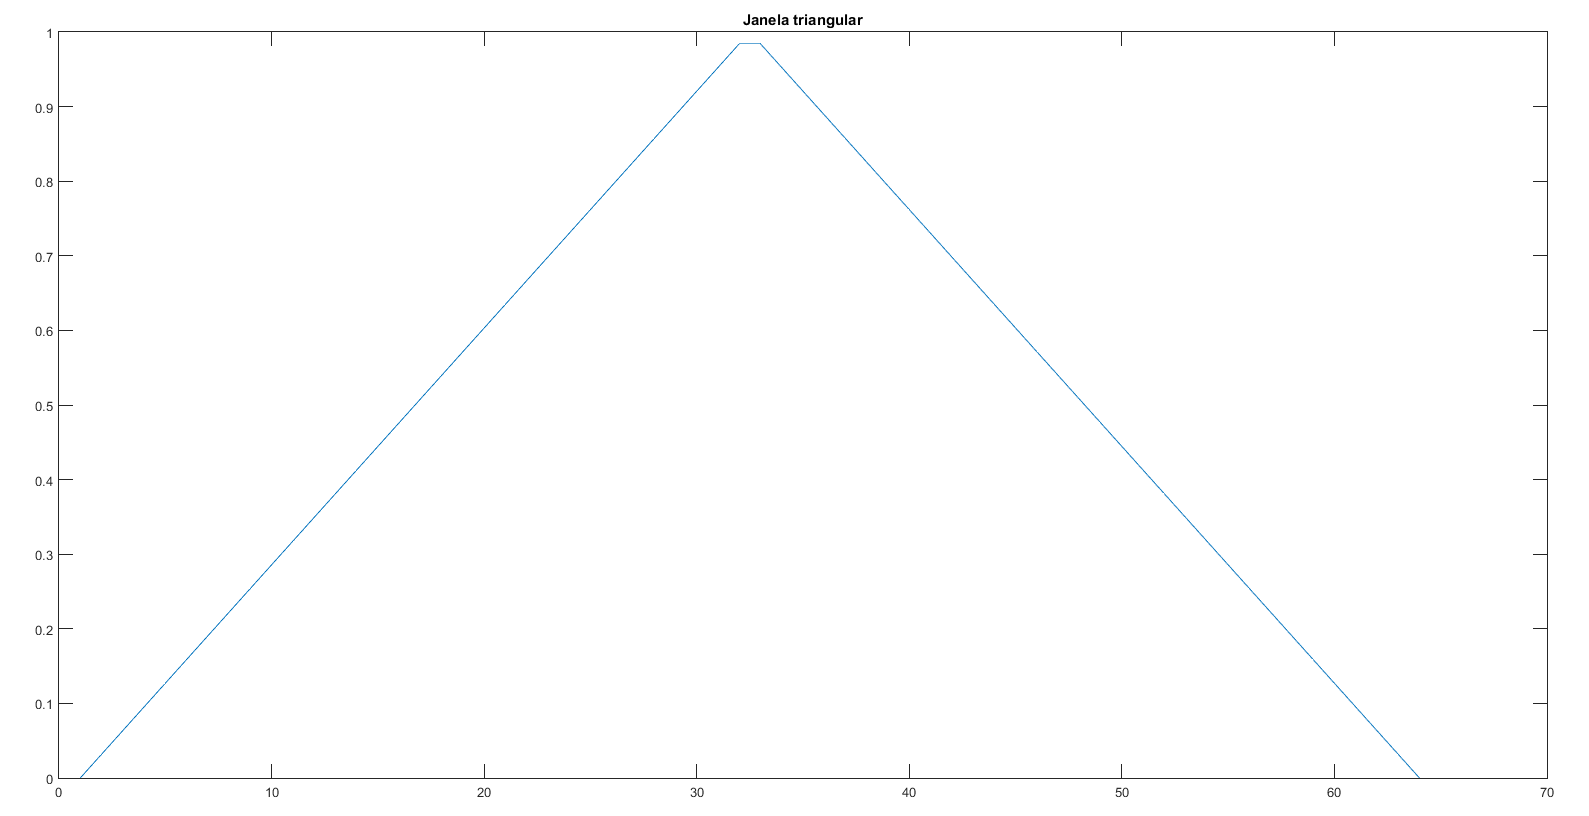
\includegraphics[width=0.9\textwidth]{figuras/f4.png}
    \caption{legenda aqui}
    \label{fig:f4}
\end{figure}

\begin{figure}[h]
    \centering
    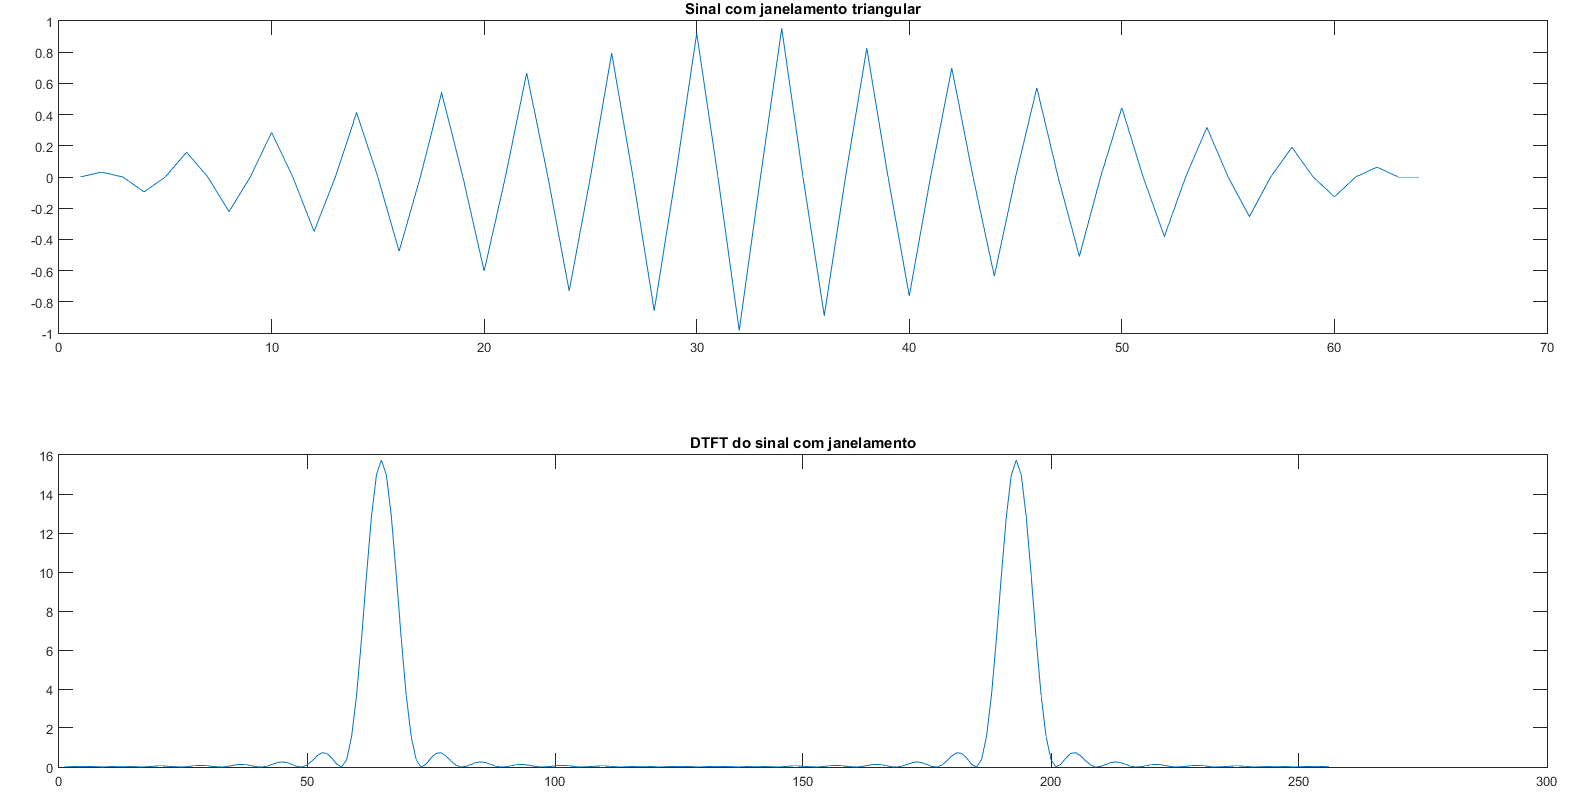
\includegraphics[width=0.9\textwidth]{figuras/f3.png}
    \caption{legenda aqui}
    \label{fig:f3}
\end{figure}

\begin{figure}[h]
    \centering
    \includegraphics[width=0.9\textwidth]{figuras/findent.png}
    \caption{legenda aqui}
    \label{fig:findent}
\end{figure}

\begin{figure}[h]
    \centering
    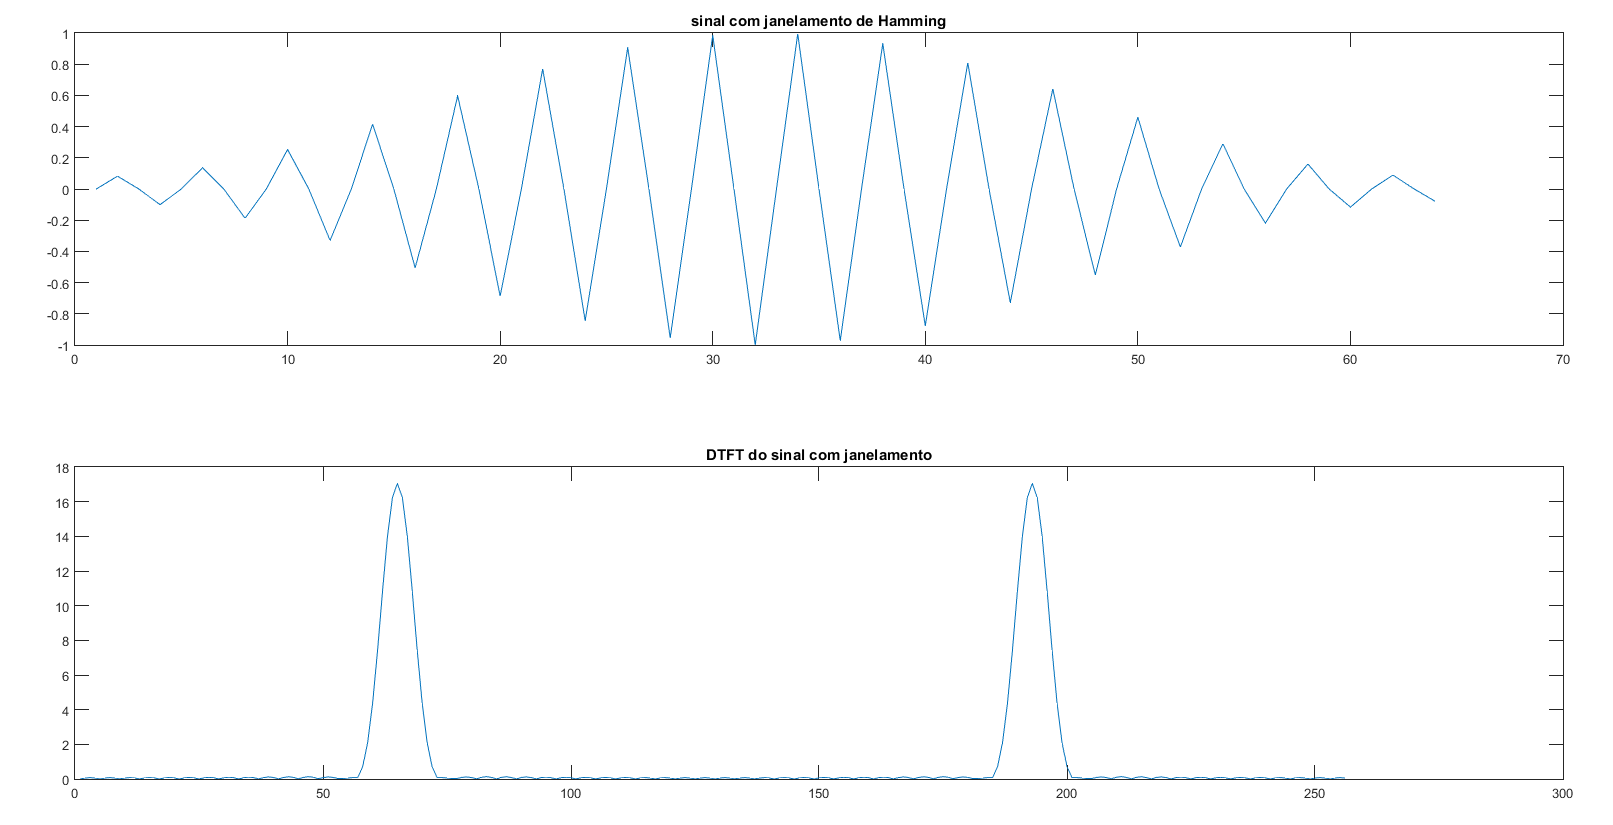
\includegraphics[width=0.9\textwidth]{figuras/f1.png}
    \caption{legenda aqui}
    \label{fig:f1}
\end{figure}

\section{Análise de Prony}
A análise de Prony foi desenvolvida em 1795 de modo a explicar a espanção de gases. Ela se assemelha em parte a DFT, entretanto se propõe a ajustar uma soma de exponenciais complexas amortecidas a uma sequência de dados igualmente espaçados, ao passo de que a DFT apenas estima as exponeciais complexas e em subdivisões predeterminadas da frequência de amostragem. A análise de prony não é somente uma técnica de análise de sinais, mas também de indentificação de sistemas amplamente utilizada em sistemas de potência, área biomédica, processamento de fala, decaimento radioativo entre outas. 
A análise de Prony é conhecida por não se comportar muito bem quando um sinal contém ruído, a técnica não faz distinção entre sinal e ruído, e também ajusta as exponenciais ao ruído presente.
Seguindo o proposto em [3], temos o seguinte para um sinal $y[k]$ imaginando M exponenciais para se ajustarem a indentM amostras, respeitando o teorema da amostragem:

\Large
\begin{equation}
    y[k]=\sum_{m=1}^{M}A_me^{(\alpha_m+jindent\pi f_m)(k-1)\Delta t +j\sigma_m}\;,\;k=1,indent,...,indentM
\end{equation}
\normalsize

\indent Onde $fm$ é a frequência das exponenciais, $\Delta t$ é o tempo de amostragem, $\alpha _m$ é o coeficiente de amortecimento, e $\sigma _m$ é o ângulo de defasagem. Para o método proposto, estamos apenas interessados em saber quais são as frequências presentes no sinal. Se imaginamos nosso sistema sendo auto regressivo (AR) de ordem M, temos que em qualquer instante de $k$ é possível prever o valor $y[k]$ considerando apenas as M amostras anteriores deste mesmo sinal. Podemos então montar uma equação de diferenças, que neste caso também é um modelo de predição linear[4]:

\begin{equation}
    y[k]=\sum_{m=1}^{M}a_m y[k-m]
\end{equation}

É sabido que exponenciais complexas são soluções para tal modelo. Se tivermos em mãos os valores dos coeficientes $a$ podemos montar o polinômio característico da equação e as raízes deste polinômio (exponenciais complexas) são soluções para nosso problema. De posse dos coeficientes $a$ devemos então encontrar as raízes do polinômio seguinte:
\begin{equation}
    P(z)=z^M-a_1z^{M-1}-...-a_Mz^0
\end{equation}

\indent Como os coeficientes $a$  são reais, as raízes complexas estão em pares complexos conjugados, desta maneira cada par complexo representa uma possível senóide já que $cos(wt)=\frac{e^{jwt}+e^{-jwt}}{indent}$:
\begin{equation}
    f_m=atan(Im\{z_m\}/Re\{z_m\})indent\pi fs
\end{equation}

\indent Onde $_zm$ é uma das raízes e $fs$ é a frequência de amostragem.
\indent Reparemos que as frequências $f_m$ são frequências de possíveis soluções do sistema, não necessariamente elas estarão presentes. Qualquer combinação linear dessas senióides também é solução do sistema AR planteado. Para encontrar a forma da solução real, é  necessário fazer uso das condições iniciais conhecidas de nosso sistema. No caso, as próprias amostras $y[k]$ as quais temos acesso.

\indent Os coeficientes de amortecimento $\alpha_m$ são o módulo das raízes complexas que encontramos. E se alguma raíz não é complexa, isto somente significa que uma exponencial é solução para nossa equação.
\begin{equation}
    \alpha_m=|zm|
\end{equation}
\subsection{Solução do modelo de predição linear}

Existem diversas formas de solucionar um modelo deste tipo, apresentaremos algumas opções abaixo[9]:

\subsubsection{Sistema linear}

Conhecendo os valores $y[k]$ que são amostras de nosso sistema analisado, podemos montar um sistema linear considerando a equação anterior:
\begin{equation}
    y[k]=\sum_{m=1}^{M}a_m y[k-m]
    
    \begin{bmatrix}
    y[k-1] & y[k-indent] & \dots & y[k-M] \\
    y[k-indent] & y[k-3] & \dots & y[k-M-1] \\
    \vdots & & & \vdots\\
    y[k-M] & y[k-M-1] & \dots & y[k-indentM+1]
    \end{bmatrix}
    \begin{bmatrix}
    a_1 \\ a_indent \\ \vdots \\ a_M
    \end{bmatrix}
    =
    \begin{bmatrix}
    y[k] \\ y[k-1] \\ \vdots \\ y[k-M+1]
    \end{bmatrix}
    
\end{equation}

Ou de forma simplificada:

\begin{equation}
    \boldsymbol{Y_k}\boldsymbol{a}=\boldsymbol{y_k}
\end{equation}

A forma mais simples de resolver este sistema é inverter a matriz $\boldsymbol{Y_k}$:

\begin{equation}
    \boldsymbol{a}=\boldsymbol{Y_k}^{-1}\boldsymbol{y_k}
\end{equation}

Um dos problemas com esta solução é que ela é computacionalmente custosa, já  que não está implementada de maneira recursiva, mas pior que isso é o fato de que normalmente temos ruído em nosso sistema, e desta maneira estamos ajustando os valores de $\boldsymbol{a}$ ao ruído também, o que em geral não é o desejado, e em nosso caso, certamente não é. Desta forma, cada vez que calculamos o vetor $\boldsymbol{a}$, ele pode sair completamente diferente do anterior, nos levando a estimações equivocadas. Modelando $y[k]$ como:
\begin{equation}
    y[k]=\sum_{m=1}^{M}a_m y[k-m]+\xi_k
\end{equation}

Em que $\xi_k$ é ruído branco, temos um modelo estocástico de nosso sinal, que nos possibilita pensar em soluções mais arrojadas. 

\subsection{Filtros adaptativos}

\indent O Elemento linear adaptativo, ou filtro FIR adaptativo, também chamado de ADALINE, é uma rede neural artificial composta de uma única camada e com função de ativação linear. Sendo $\boldsymbol{x}$ as entradas, $\boldsymbol{w}$ os pesos, $b$ o valor de bias, o ADALINE pode ser implementado matricialmente da seguinte maneira:


\begin{equation}
    y=
    \begin{bmatrix}
    x_{1} & x_{indent} & x_{3} & \dots & x_{n} \\
    \end{bmatrix}
    *
    \begin{bmatrix}
    w_{1}  \\
    w_{indent}  \\
    \vdots  \\
    w_{n} 
    \end{bmatrix}
    + b = \boldsymbol{x}*\boldsymbol{w}+b
\end{equation}

\begin{figure}[h]
    \centering
    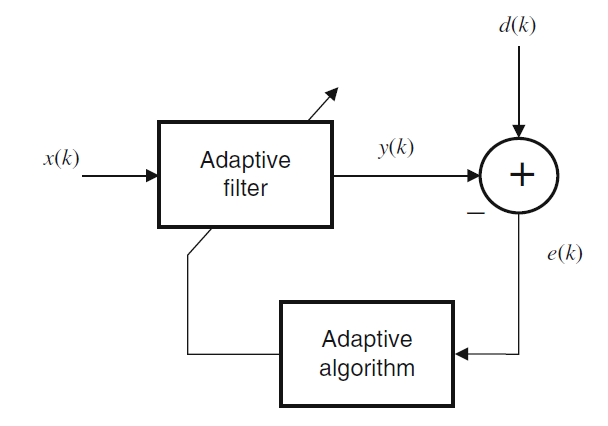
\includegraphics[width=0.9\textwidth]{figuras/fA.png}
    \caption{legenda aqui}
    \label{fig:filtroAdaptativo}
\end{figure}

\indent Filtros adaptativos são considerados sistemas não lineares, portanto a análise de seu comportamento é mais complexa que de a filtros com coeficientes fixos. Por outro lado, pelo fato de serem auto-projetados, por um ponto de vista mais prático, eles podem ser considerados menos complicados que os convencionais em termos de projeto[6].

\indent O desenho usual de um filtro adaptativo pode ser visto na figura \ref{fig:filtroAdaptativo}, onde $k$ é o número da iteração, $x(k)$ é a entrada do filtro, $y(k)$ é o sinal de saída, $d(k)$ é o valor de referência e $e(k)=d(k)-y(k)$ é o valor de erro, necessário para o algoritmo de adaptação do filtro. O algoritmo de adaptação é o prcesso usado para ajustar os coeficientes do filtro de modo a minimizar o erro de acordo com os critétios preestabelecidos. A escolha do algoritmo determina muitos aspectos do processo de adaptação, como a existência de soluções subótimas e complexidade computacional.

\subsection{Adaptação via gradiente descendente}

Uma das formas mais antigas e consagradas de otimizar uma função dentro dos métodos clássicos é seguir a direção do gradiente desta função, com relação as variáveis de interesse, para atualizar os valores destas variáveis de forma iterativa.

Consideremos um sistema discriminado pela série temporal $u[n] \space n=0,1,indent..$ e um filtro de resposta impulsiva real $w_0, w_1 ... w_{M-1}$:
\begin{equation}
    y[n]=\sum_{k=0}^{M-1}u[n-k]w_k
\end{equation}
Todo este desenvolvimento pode ser feito de maneira bastante similar considerando entradas complexas e filtros com coeficientes complexos, mas por questões de simplicidade estaremos focando no caso em que ambos são reais. Imaginemos que desejamos que a saída deste filtro seja uma outra série temporal igualmente real $d[n]$, assim nosso erro seria:
\begin{equation}
    e[n]=d[n]-y[n]    
\end{equation}

Considerando o caso de $u$ estocástico, $e[n]$ é uma variável aleatória. Gostaríamos então de minimizar a esperança de $e^indent[n]$, definimos então nossa função de custo:
\begin{equation}
    J=E[e^indent[n]]=E[(d[n]-y[n])^indent]   
\end{equation}

Definindo nosso operador gradiente $\nabla_k$:
\begin{equation}
    \nabla_k J=-indent E[e[n]u[n-k]]   
\end{equation}

Se queremos encontrar o ótimo com relação a esta função de custo, $\nabla_k J$ deve ser igual a zero para todo $k$, como a esperança do produto de duas variáveis aleatórias é sua correlação, $u[n-k]$ e $e[n]$ devem estar descorrelacionadas para todo $k$. A este resultados chamamos princípio da ortogonalidade. Um corolário deste princípio é que $y$ também deve ser ortogonal, ou descorrelacionada com $e[n]$.

\indent É mais conveniente para nó trabalhar com a notação matricial destes resultados. Ao vetor coluna que contém as variáveis aleatórias $u[n-k]$, de k=0 a K=M-1, lhe chamamos $\boldsymbol{u}_n$, ao vetor de coeficientes $w$, igualmente:

\begin{equation*}
    \boldsymbol{u}_n=
    \begin{bmatrix}
        u[n] & u[n-1] & \dots & u[n-M+1]
    \end{bmatrix}^T
\end{equation*}
\begin{equation*}
    \boldsymbol{W}_n=
    \begin{bmatrix}
        w_0 & w_1 & \dots & w_{M-1}
    \end{bmatrix}^T
\end{equation*}
Desenvolvendo nossa equação anterior, podemos obter:

\begin{equation}
    \nabla J=-indent E[e[n]\boldsymbol{u}_n]=indentE[\boldsymbol{u}_n\boldsymbol{U}^{T}_n\boldsymbol{W}-d[n]\boldsymbol{u}_n]   
\end{equation}

Desta última equação, destacamos que $E[d[n]\boldsymbol{U}_n]$ é o vetor de correlação cruzada entre $d[n]$, que chamaremos de $\boldsymbol{r_{du}}$ e as amostras atrasadas do sinal de entrada.Destacamos também que $E[\boldsymbol{U}_n\boldsymbol{U}^{T}_n]$, a qual chamaremos $\boldsymbol{R_{uu}}$, é a matriz MxM de autocorrelação do mesmo sinal. Sendo assim, escrevemos agora:

\begin{equation}
    \boldsymbol{R}_{uu}\boldsymbol{w}-\boldsymbol{r}_{du}=0
\end{equation}

De onde podemos concluir que o vetor coeficientes ótimos $\boldsymbol{w}_{opt}$ é:

\begin{equation}
    \boldsymbol{w}_{opt}=\boldsymbol{R}_{uu}^{-1}\boldsymbol{r}_{du}
\end{equation}

Se $u$ é um processo estacionário em sentido amplo, então podemos coletar amostras suficientes para fazer uma boa estimação das matrizes acima, encontrando assim um filtro muito mais apropriado para nossos propósitos. Desta maneira, é possível estimar o conteúdo espectral de $u$ com precisão. Reparemos que este método não é propriamente um gradiente escendente já que encontramos a solução em um passo apenas.

\indent A solução acima tem sua utilidade, entretanto, se a natureza do sinal mudar, não teremos mais uma boa aproximação do mesmo, neste caso, é melhor resolver estas equações de forma recursiva, de modo que o filtro possa se adaptar constantemente à mudanças ocorridas.  

\subsection{O algoritmo LMS}

Para atualizar o vetor de pesos $\boldsymbol{w}_n$ na direção oposta a do gradiente, definimos um coeficiente de aprendizagem $\mu$. A cada iteração vamos fazer o seguinte:

\begin{equation*}
    \boldsymbol{w}_{n}=\boldsymbol{w}_{n-1} - \mu \nabla J
\end{equation*}
\begin{equation}
    \boldsymbol{w}_{n}=\boldsymbol{w}_{n-1} + \mu(\boldsymbol{r}_{du}-\boldsymbol{R}_{uu} \boldsymbol{w}_{n+1})
\end{equation}

O que diferencia o LMS de outros métodos de gradiente descendente é a forma de estimar as matrizes $\boldsymbol{R}_{uu}$ e $\boldsymbol{r}_{du}$. Vamos estimâ-las da seguinte forma:

\begin{equation}
    \boldsymbol{\hat{R}}_{uu}=\boldsymbol{u}_n \boldsymbol{u}_{n}^T
\end{equation}
\begin{equation}
    \boldsymbol{\hat{r}}_{du}=\boldsymbol{u}_n d[n]
\end{equation}

O que pode soar uma heresia, mas faz sentido se pensarmos que apenas temos M amostras de sinal.

\subsection{O algoritmo NLMS}

Uma melhoria no algoritmo anterior pode ser proposta. Se multiplicamos a parte que está entre parênteses na equação XX:

\begin{equation}
    \boldsymbol{w}_{n}=\boldsymbol{w}_{n-1} + \mu \boldsymbol{R}_{uu}^{-1}(\boldsymbol{r}_{du}-\boldsymbol{R}_{uu} \boldsymbol{w}_{n+1}) = \boldsymbol{w}_{n-1} + \mu(\boldsymbol{w}_{opt} - I \boldsymbol{w}_{n-1}) = \boldsymbol{w}_{opt}
\end{equation}

Em teoria, nosso algoritmo convergiria em apenas uma iteração. Resta apenas o empecilho de que estimar tal matriz. Com estimador que tínhamos antes isto não é possível, porque a matriz estimada $\boldsymbol{\hat{R}}_{uu}$ não é inversível por ser o produto de dois vetores. Mas podemos fazer uma aproximação da forma $\boldsymbol{\hat{R}}_{uu} + \boldsymbol{I} \epsilon$. Que certamente é inversível e pode nos dar uma inversa útil, para valores pequenos de $\epsilon$. E após alguma álgebra[10], que pode ser encontrada em [9], chegamos ao seguinte:

\begin{equation}
    \boldsymbol{w}_{n}=\boldsymbol{w}_{n-1} + \mu \frac{\boldsymbol{u}_{n}}{|\boldsymbol{u}_{n}|^indent + \epsilon }(d[n]-\boldsymbol{u}_{n} \boldsymbol{w}_{n-1}) =\boldsymbol{w}_{n-1} + \mu \frac{\boldsymbol{u}_{n}}{|\boldsymbol{u}_{n}|^indent + \epsilon }e[n]
\end{equation}

A este algoritmo chamamos LMS normalizado, ou NLMS. Há ainda o estudo de convergência para valores pequenos de $\mu$, que também pode ser encontrado em [6][9], tanto para o LMS quanto para o NLMS. Mas de modo geral o NLMS deve convergir respeirada todas as condições estabelecidas anteriormente e escolhendo valores de $\mu<1$.

\section{RLS}

\indent O método RLS (\textit{Recursive Least Squares}), ou mínimos quadrados recursivo, é um método de adaptação que visa a minimização da soma dos quadrados da diferença entre o sinal de referência e o sinal de saída do filtro em questão (o erro). O RLS pode ser obtido apartir do LMS (\textit{Least Mean Squares}). O RLS é conhecido por possuir rápida convergência, tendo boa performance em sistemas variantes no tempo, como o caso de nosso interesse. Isto vem ao custo de certa complexidade computacional aliada a problemas de estabilidade[6].

\indent Voltando ao modelo do filtro adaptativo da seção anterior, vamos definir $\boldsymbol{x}(k)$ como o vetor contendo $N$ amostras atrasadas de nosso sinal de entrada, ou seja $x(k)$. Assim:

\begin{equation}
    \boldsymbol{x}(k)=
    \begin{bmatrix}
        x(k-1) & x(k-indent) & \dots & x(k-N) \\
    \end{bmatrix}
\end{equation}

\indent Sendo N a ordem do filtro. Da mesma maneira, podemos definir $\boldsymbol{w}(k)$ como o vetor contendo os coeficientes do filtro na $k$ ésima iteração. Assim:
\begin{equation}
    \boldsymbol{w}(k)=
    \begin{bmatrix}
    w_{1}(k)  \\
    w_{indent}(k)  \\
    \vdots  \\
    w_{N}(k) 
    \end{bmatrix}
    
\end{equation}

\indent A função objetivo para o RLS é determinística e dada por:

\Large
\begin{equation}
    \xi(k)=\sum_{i=0}^{k}\lambda^{k-i}\varepsilon^indent(i)
    =\sum_{i=0}^{k}\lambda^{k-i}[d(i)-\boldsymbol{x}(k)*\boldsymbol{w}(k)]
\end{equation}
\normalsize

\indent Onde $\varepsilon$ é o erro a posteriori no instante $i$. O parâmetro $\lambda$ é um fator de peso exponencial que deve ser escolhido entre 0 e 1, de modo que $0 << \lambda < 1$. $\lambda$ representa o fator de esquecimento do erro, quanto menor seu valor, menor será a influência das amostras passadas sobre a atualização atual.

\indent Após alguma álgebra que pode ser encntrada em [6], temos o seguinte:

\Large
\begin{equation}
    \boldsymbol{w}(k)=\boldsymbol{S}_d(k)*\boldsymbol{p}_d(k)
\end{equation}


\begin{equation}
    \boldsymbol{S}_d=\lambda^{-1}\Bigg[\boldsymbol{S}_d(k-1)-\frac{\boldsymbol{S}_d(k-1)\boldsymbol{x}^T(k)\boldsymbol{x}(k)\boldsymbol{S}_d}{\lambda+\boldsymbol{x}(k)\boldsymbol{S}_d(k)\boldsymbol{x}^T(k)}\Bigg]
\end{equation}

\begin{equation}
    \boldsymbol{p}_d(k)=\lambda \boldsymbol{p}_d(k-1)+d(k)*\boldsymbol{x}(k)
\end{equation}
\normalsize

\indent Boas recomendações de inicialização de $\boldsymbol{S}_d$ e $\boldsymbol{p}_d$ são $\boldsymbol{S}_d=\delta \boldsymbol{I}$ e $\boldsymbol{p}_d=[0\;0\;...\;0]^_T$. Nas quais $\delta$ pode ser o inverso da potência estimada do sinal.

\section{PLL}

\indent Um Phase Locked Loop digital, assim como sua versão analógica, visa determinar os parâmetros de um processo estocáscico como uma onda senoidal. Desta forma o PLL tenta extrair parâmetros de Amplitude, fase e frequência. Temos diversas variantes digitais e analógicas[7], a variante utilizada neste trabalho foi proposta por Ziarani em indent004[8]. Uma breve demostração será realizada abaixo.
\indent Seja $u(t)$ uma função variante no tempo, e $y(t)=Asin\phi(t)$ um sinal periódico senoidal sendo A a amplitude do sinal e $\phi(t)$ sua fase, tendo este sinal uma frequência constante, podemos escrever $\phi(t)=wt+\delta$, sendo $w$ igual a frequência e $\delta$ um valor de fase constante. Podemos escrever de maneira mais geral:

\begin{equation}
    u(t)=\sum_{i=0}^{\infty}A_i sin\phi_i(t)\space+\space n(t)
\end{equation}

Onde $n(t)$ representa um distúrbio, como um ruído. Na realidade, todos os parâmetros podem variar com o tempo, é conveniente escrever então um conjunto $\Psi(t)=[A(t), w(t), \delta(t)]$ o qual contém todos os parâmetros de um possível sinal $y(t)$.

Definimos a função $d$:
\begin{equation}
    d^indent(t,\Psi(t))=[u(t)-y(t,\Psi(t))]^indent=e^indent(t)
\end{equation}

Assim sendo o conjunto $\Psi(t)$ ótimo o que minimiza a função $d^indent$ que adotaremos como função de custo $J(\Psi(t),t)$. Os parâmetros $\Psi(t)$ podem ser estimados por meio de gradiente descendente.

\begin{equation}
    \frac{d\Psi(t)}{dt}=-\boldsymbol{\mu}\frac{\partial J(\Psi(t),t)}{\partial \Psi(t)}
    \
\end{equation}

\begin{equation}
    \boldsymbol{\mu}=
    \begin{bmatrix}
        m_1 && 0 && 0 \\
        0 && m_indent && 0 \\
        0 && 0 && m_3
    \end{bmatrix}
\end{equation}

Com $\frac{d\Psi(t)}{dt}$ denotando o vetor na dierção do qual são atualizados os valores de $\Psi(t)$ a cada iteração. E $\boldsymbol{\mu}$ a matriz diagonal contendo as constantes de atualização referentes a cada parâmetro. Como estaremos lidando com estimações agora, usaremos a notação $\hat{\Psi}(t)$:

\begin{equation}
    \begin{bmatrix}
        \frac{d\hat{A}(t)}{dt} \\
        \frac{d\hat{w}(t)}{dt}\\
        \frac{d\hat{\delta}(t)}{dt}
    \end{bmatrix}
    =-\boldsymbol{\mu}
    \begin{bmatrix}
    \frac{\partial e^indent(t)}{\partial \hat{A}} \\
    \frac{\partial e^indent(t)}{\partial \hat{w}} \\
    \frac{\partial e^indent(t)}{\partial \hat{\delta}}
    \end{bmatrix}
\end{equation}

Podemos obter então o seguinte:
\begin{equation}
    \frac{d\hat{A}(t)}{dt}=indentm_1e(t)sin(\int_{0}^{t}\hat{w}(\tau)d\tau\space+\space\hat{\delta}(t))
\end{equation}
\begin{equation}
    \frac{d\hat{w}(t)}{dt}=indentm_indente(t)\hat{A}(t)tcos(\int_{0}^{t}\hat{w}(\tau)d\tau\space+\space\hat{\delta}(t))
\end{equation}
\begin{equation}
    \frac{d\hat{\delta}(t)}{dt}=indentm_3e(t)\hat{A}(t)cos(\int_{0}^{t}\hat{w}(\tau)d\tau\space+\space\hat{\delta}(t))
\end{equation}
\begin{equation}
    \frac{d\hat{\phi}(t)}{dt}=\hat{w}(t)+\frac{\hat{\delta}(t)}{dt}
\end{equation}

Por conta do fator temporal $t$ que aparece solto na equação referente a $\hat{w}$, esse sistema é variante no tempo, o que o torna instável. No entanto uma solução heurística é substituir $t$ por uma constante $m4$, que pode ser absorvida pela constante $mindent$, tornando o sistema invariante no tempo e fazendo com que este sistema de equações seja útil na prática. Desta maneira obtemos o seguinte:
\begin{equation}
    \frac{d\hat{A}(t)}{dt}=indent\mu_1e(t)sin(\int_{0}^{t}\hat{w}(\tau)d\tau\space+\space\hat{\delta}(t))
\end{equation}
\begin{equation}
    \frac{d\hat{w}(t)}{dt}=indent\mu_indente(t)\hat{A}(t)tcos(\int_{0}^{t}\hat{w}(\tau)d\tau\space+\space\hat{\delta}(t))
\end{equation}
\begin{equation}
    \frac{d\hat{\phi}(t)}{dt}=\hat{w}(t)+indent\mu_3e(t)\hat{A}(t)cos(\int_{0}^{t}\hat{w}(\tau)d\tau\space+\space\hat{\delta}(t))
\end{equation}

Usando o método \italic{Euler Forward}:

\begin{equation}
    A[n+1]=A[n]+\mu_1T_s e[n]sen(\phi(t))
\end{equation}
\begin{equation}
    w[n+1]=w[n]+\mu_indentT_s e[n]cos(\phi(t))
\end{equation}
\begin{equation}
    \phi[n+1]=\phi[n] + T_s w[n] + \mu_3T_s e[n]cos(\phi(t))
\end{equation}

Desta forma obtemos o conjunto de equações discretas que utilizaremos para rastrear frequências no restante do trabalho.

\end{document}